%%%--------------------------------%%%
%%% UC2
%%%--------------------------------%%%

\newpage
% UC2 ====================================================
\subsubsection{Use Case Specification: \ac{UC}2 Project Access Management CRUD}
\label{sec:domainBbc}

\begin{wrapfigure}{r}{0.3\textwidth}
	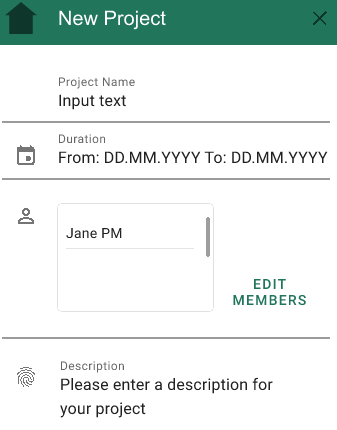
\includegraphics[width=0.3\textwidth]{Assets/UC_Screenshots/UC2S.png}
	\caption{Use Case 2: Mock Prototype}
	\label{fig:useCase2Detail}
\end{wrapfigure}


\paragraph*{Description}\mbox{}\\
This use case specifies how projects are being created, updated, deleted and are used for grouping a pool of users and risks.
The fields in the list below are required for the project creation:


\begin{itemize}
	\vspace{-3mm}
	\setlength\itemsep{-1em}
	\item projetc name (String)
	\item project description (String)
	\item start date (Date)
	\item end date (Date)
\end{itemize}
Besides the required fields the project owner can set the following field while updating a project:
\begin{itemize}
	\vspace{-3mm}
	\setlength\itemsep{-1em}
	\item project members (Strings: Usernames, E-Mails)
\end{itemize}

\paragraph*{Basic Flow} \mbox{}\\
\noindent
New Project:
\begin{itemize}
	\vspace{-3mm}
	\setlength\itemsep{-1em}
	
	\item The user is currently on the project page and clicks the "new project" button and fills in the required fields.
	\item Then clicks on the "create" button to send the input to the server.
	\item If the users input fulfills the criteria of a name, description and time span, the project will be created on the server and be available in the project list.
\end{itemize}

\noindent
Update Project: 
\begin{itemize}
	\vspace{-3mm}
	\setlength\itemsep{-1em}
	\item The user opened the detailed project page by clicking on it on the project list and then clicks the "edit" button.
	\item After updating the fields the user, to be more precise the project owner, intended to change, those updated fields are send to the server by clicking the "save" button.
	\item If the updated fields fulfill their criterias, those fields are updated on the server and in the user interface.
\end{itemize} 
Adding users while updating a project is the basis to work on risks together as described in chapter \ref{sec:domainBbd}

\noindent
Delete Project:
\begin{itemize}
	\vspace{-3mm}
	\setlength\itemsep{-1em}
	\item The project owner opened the detailed project page by clicking on it on the project list and then clicks the "edit" button.
	\item The owner then clicks on the "delete" button. 
	\item After typing in the users password, the request to delete the project will be send to the server once the "delete" button is clicked.
	\item If the given password match the owner's password the project, including all related risks, is being deleted on the server and removed from the project list in the user interface.
\end{itemize}

\newpage
\subparagraph{Activity Diagram}\mbox{}\\
\begin{figure}[H]
	\centering
	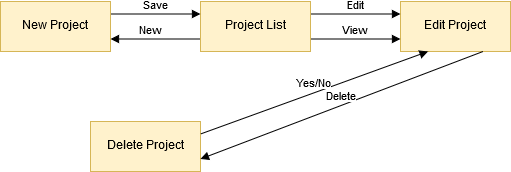
\includegraphics[width=0.9\textwidth]{Content/Domain/UC2ProjectCRUDactivitydiagram.png}
	\caption{Activity Diagram \ac{UC}2 Project CRUD}
	\label{fig:activityDiagramUC2}
\end{figure}

\paragraph*{Alternative Flows}\mbox{}\\

\noindent
Invalid input: 
\begin{itemize}
	\vspace{-3mm}
	\setlength\itemsep{-1em}
	\item Like chapter \ref{sec:domainBbb} "Invalid Input", but for project creations and updates.
\end{itemize}

\noindent
Invalid user credentials:
\begin{itemize}
	\vspace{-3mm}
	\setlength\itemsep{-1em}
	\item Like chapter \ref{sec:domainBbb} "Invalid user credentials", but for project deletion.
\end{itemize}

\paragraph*{Special Requirements and Preconditions}\mbox{}\\
Generally, the user who created the project is automatically the project owner.
\begin{enumerate}
	\vspace{-3mm}
	\setlength\itemsep{-1em}
	\item The user has to be logged in to create a project. 
	\item The user has to be the owner of a project to edit it.
\end{enumerate}

\paragraph*{Postconditions and Persistance}\mbox{}\\
Mentionable postconditions are:
\begin{enumerate}
	\vspace{-3mm}
	\setlength\itemsep{-1em}
	\item When deleting a project, the project including all related risks can not be restored.
	\item After creating a project and adding users, users will be able to access it and create risks within.
\end{enumerate}

\noindent
The persistence guidelines are: 
\newline
\noindent
All mentioned basic flows above create POST requests to the server and additionally, if the fields meet their criterias the data will be persisted.